\title{Sorting Algorithms in Practice}
\author{
        Donner Hanson \\
                Schmidt College of Science and Technology\\
        Chapman University\\
        Department of Computer Science\\
}
\date{\today}

\RequirePackage{filecontents}
\begin{filecontents}{\jobname.bib}
@book{key,
author = {Author, A.},
year = {2001},
title = {Title},
publisher = {Publisher},
}
\end{filecontents}

\documentclass[12pt]{article}
\usepackage{url}
\usepackage{graphicx}
\graphicspath{ {\string~/Desktop/} }
\begin{document}
\maketitle

\begin{abstract}
This paper will discuss the differences of the sorting algorithms Bubble Sort, Selection Sort, Insertion Sort, Merge Sort, and Recursive Quick Sort.
\end{abstract}

\paragraph{Outline}
This report is organized as follows:\newline
Section~\ref{intro} : Introduction\newline
Section~\ref{bsresults} : Bubble Sort\newline
Section~\ref{ssresults} : Selection Sort\newline
Section~\ref{isresults} : Insertion Sort\newline   
Section~\ref{msresults}: Merge Sort\newline   
Section~\ref{qsresults} : Quick Sort\newline   
Section~\ref{conclusions} : Conclusion

\section{Introduction}\label{intro}

\begin{figure}[htbp]
\centering
  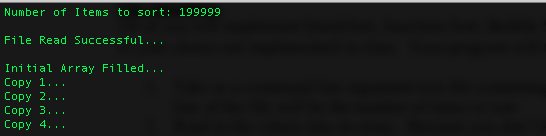
\includegraphics[width=.7\linewidth]{fread.png}
 \caption{Number of Items Sorted}
\end{figure}

Assignment 6 is a demonstration of how differing sort algorithms work. To construct the txt file included I used the standard distribution functionality from C++11. I generated random doubles in a range and output to the txt file. The program also skips any whitespace and characters that may be included in the data to sort.   
The internal data structure I created to hold the values of the data to sort is a custom Dynamic Array class. When the base array has reach its max length it is copied to a new array, pointers are swapped, and the old array deleted.
To time the sorting of the data I made use of the C++11 std::chrono library to calculate the time of each sort in microseconds.
 

\section{Bubble Sort Results}\label{bsresults}
Bubble sort is great for a quick solution to a small set of numbers. However, when the size of the data reaches into the hundreds of thousands, or millions, my hardware (2012 Macbook Pro) runs at max capacity slowing to a sluggish pace. This was my first time sorting large amounts of data so I was quite shocked to see that I could actually get some chores done and eat dinner while I waited for the results while waiting for this O(n\textsuperscript{2}) algorithm to finish.\newline

\begin{figure}[htbp]
\centering
  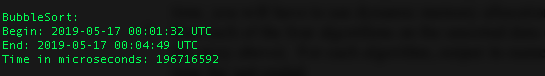
\includegraphics[width=.7\linewidth]{bs.png}
 \caption{Bubble Sort Results}
\end{figure}

\section{Selection Sort Results}\label{ssresults}
Selection sort seemed to run slightly faster than bubble sort with large sets of data but the change was not nearly that remarkable. Again, an O(n\textsuperscript{2}) algorithm has surprised me.\newline

\begin{figure}[htbp]
\centering
  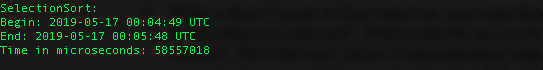
\includegraphics[width=.7\linewidth]{ss.png}
 \caption{Selection Sort Results}
\end{figure}

\section{Insertion Sort Results}\label{isresults}

Insertion sort actually seemed to run far quicker than expected - especially after watching Bubble and Selection sorts run at a snails pace, even though Insertion Sort is also considered O(n\textsuperscript{2}). This could have been due to the uniformly distributed random numbers that were loaded into the doubles.txt file being somewhat sorted. However, the sort still took a while. \newline

\begin{figure}[htbp]
\centering
  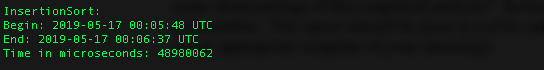
\includegraphics[width=.7\linewidth]{is.png}
 \caption{Insertion Sort Results}
\end{figure}


\section{Merge Sort Results}\label{msresults}
Merge sort wowed me. It brought a better understanding of what an O(nlogn) algorithm can complete compared to the previous algorithms. In under a second, 199999 items had been sorted. \begin{figure}[htbp]
\centering
  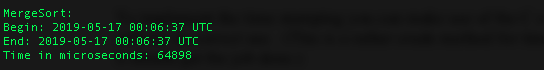
\includegraphics[width=.7\linewidth]{ms.png}
 \caption{Merge Sort Results}
\end{figure}

\section{Quick Sort Results}\label{qsresults}
To my surprise, Quick Sort was, well... quick! Again, impressed by the speed of the recursive algorithms.
\begin{figure}[htbp]
\centering
  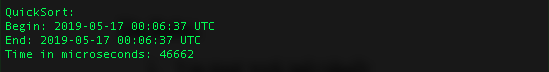
\includegraphics[width=.7\linewidth]{qs.png}
 \caption{Quick Sort Results}
\end{figure}

\section{Conclusions}\label{conclusions}
Recursion is useful and, given the right environment and specs of data, should be embraced for efficiency. I was pleasantly surprised by the efficiency of Quick Sort as well as Merge Sort and will be implementing them more frequently where appropriate.

%\cite{GEEKSQS}
%\bibliography{simple} any references with URLS fails
%\bibliographystyle{anystyleiputherefails}

\end{document}
